\documentclass{article}

\usepackage{a4}
\usepackage{amsmath}
\usepackage{amssymb}
\usepackage{ctex}
\usepackage{booktabs}
\usepackage{graphicx}
\usepackage{subfigure}
\usepackage{subcaption}
\usepackage{float}
\usepackage{hyperref}
\usepackage{xurl}
\usepackage{enumitem}
\usepackage{array}
\usepackage{longtable}
\usepackage{multirow}
\usepackage{fvextra}

\hypersetup{colorlinks=true,linkcolor=black,urlcolor=blue,citecolor=black}
\setlist[itemize]{nosep,leftmargin=1.8em}
\setlist[enumerate]{nosep,leftmargin=1.8em}
\captionsetup{font=small}
\setlength{\emergencystretch}{3em}
\renewcommand{\arraystretch}{1.2}
\RecustomVerbatimEnvironment{verbatim}{Verbatim}{
  breaklines=true,
  breakanywhere=true,
  fontsize=\small
}
\newcommand{\sourcecode}[2]{
  \subsubsection*{#1}
  \noindent 对应文件：\path{#2}
  \VerbatimInput[
    breaklines=true,
    breakanywhere=true,
    fontsize=\small
  ]{#2}
}

\title{计算机组成原理 Project1 实验报告\\8位定点卷积--激活--池化链运算器设计}
\author{鲁昕宁 2414015}
\date{\today}

\begin{document}

\maketitle
\begin{center}
  \url{https://github.com/SidneyLu/Computer-Organization-and-Design-NKU-CS/tree/master/project1}
\end{center}

\newpage

\section{实验目标}
本实验面向边缘端 AI 场景，设计并验证一个 8 位定点卷积--激活--池化链运算器。工程目标如下：
\begin{itemize}
  \item 输入为 $5\times 5$ 的 8 位无符号灰度矩阵，像素范围为 $0\sim255$；
  \item 运算流程为 ``$5\times 5$ 输入 $\rightarrow$ $3\times 3$ 卷积层 $\rightarrow$ ReLU 激活层 $\rightarrow$ $2\times 2$ 平均池化层''；
  \item 输出为 $2\times 2$ 的 8 位特征值矩阵；
  \item 在 Vivado 环境下完成模块设计、功能仿真、综合与时序分析，并比较不同优化方案的资源占用与性能。
\end{itemize}

\section{实验环境}
本工程的开发与验证环境如下：
\begin{itemize}
  \item FPGA 器件：Xilinx Artix-7 \texttt{xc7a200tfbg676-2}
  \item RTL 语言：Verilog HDL
  \item 功能仿真：Vivado 2025.1 / XSIM
  \item 综合与时序分析：Vivado 批处理脚本 \texttt{scripts/run\_vivado\_multi\_synth.tcl}
  \item 时钟约束：\texttt{create\_clock -period 5.000 -name clk [get\_ports clk]}，即 200\,MHz
  \item I/O 约束：\texttt{set\_input\_delay 0.000} 与 \texttt{set\_output\_delay 0.000}
\end{itemize}

波形保留策略也在工程中固化：
\begin{itemize}
  \item XSIM 原始波形数据库保存在 \verb|build/xsim/waves/*.wdb|；
  \item 便于二次处理的文本波形保存在 \verb|build/xsim/waves/*.vcd|；
  \item 报告中的代表性波形图由 \verb|scripts/export_wave_figures.py| 从 VCD 自动导出到 \verb|report/figures/|。
\end{itemize}

\section{实验原理}
\subsection{卷积运算}
输入图像记为 $X$，卷积核记为 $K$。本实验采用 $3\times 3$ 卷积核对 $5\times 5$ 输入做 valid 卷积，得到 $3\times 3$ 特征图：
\[
Y(i,j)=\sum_{u=0}^{2}\sum_{v=0}^{2} X(i+u,j+v)\cdot K(u,v),\quad 0\le i,j\le 2
\]
其中像素 $X(i,j)$ 为 8 位无符号数，卷积核权重 $K(u,v)$ 为 8 位有符号数。

\subsection{ReLU 激活}
卷积输出经过 ReLU 激活后，负数被截断为 0，正数保留：
\[
R(i,j)=\max(0,Y(i,j))
\]
为保证最终结果能安全落回 8 位无符号范围，本工程进一步加入上饱和处理：若 $R(i,j)>255$，则输出钳位为 255。

\subsection{平均池化}
对 $3\times 3$ 激活图执行 $2\times 2$ 平均池化，输出 $2\times 2$ 结果：
\[
P(i,j)=\left\lfloor \frac{R(i,j)+R(i,j+1)+R(i+1,j)+R(i+1,j+1)}{4}\right\rfloor,\quad 0\le i,j\le 1
\]
由于分母恒为 4，硬件上可直接用右移 2 位实现，因此无需额外的通用除法器。

\subsection{实验分组}
本次实验实现了 5 个独立顶层：
\begin{enumerate}
  \item 串行：\texttt{cnn\_compare\_base\_top}
  \item 串行 + BoothWallace 乘法器优化：\texttt{cnn\_compare\_booth\_top}
  \item BoothWallace 乘法器优化 + SIMD：\texttt{cnn\_compare\_booth\_simd\_top}
  \item BoothWallace 乘法器优化 + SIMD + 流水线：\texttt{cnn\_compare\_booth\_simd\_pipe\_top}
  \item 第 4 组基础上换用 DSP：\texttt{cnn\_compare\_booth\_simd\_pipe\_dsp\_top}
\end{enumerate}

\section{里程碑1：核心模块设计与功能验证}
\subsection{基础模块设计}
里程碑 1 首先完成了 4 个基础模块的串行版本：
\begin{itemize}
  \item \texttt{mul8}：8 位无符号像素与 8 位有符号卷积核的乘法；
  \item \texttt{add8}：8 位无符号加法；
  \item \texttt{relu\_s20}：20 位有符号卷积结果的 ReLU 与 8 位饱和截断；
  \item \texttt{div4}：10 位无符号数除以 4 的右移实现。
\end{itemize}

下面在模块首次介绍的位置给出对应的完整 Verilog 源码。

\sourcecode{模块 \texttt{mul8} 的 Verilog 源码}{../src/baseline/mul8.v}
\sourcecode{模块 \texttt{add8} 的 Verilog 源码}{../src/baseline/add8.v}
\sourcecode{模块 \texttt{relu\_s20} 的 Verilog 源码}{../src/baseline/relu_s20.v}
\sourcecode{模块 \texttt{div4} 的 Verilog 源码}{../src/baseline/div4.v}

在此基础上，又按计划补齐了优化所需模块：
\begin{itemize}
  \item \texttt{mul8\_booth\_wallace}：真实的基 4 Booth 编码 + Wallace 树压缩 8 位乘法器；
  \item \texttt{simd\_mul8x4}：4 路 BoothWallace lane 封装；
  \item \texttt{simd\_add8x4}、\texttt{simd\_relu8x4}、\texttt{simd\_avgpool2x2\_8bit}：分别承担 4 路加法、4 路激活与池化求均值；
  \item \texttt{simd\_mul8x4\_dsp} 与 \texttt{mul8\_dsp48e1}：作为第 5 组 DSP 版的乘法实现。
\end{itemize}

\sourcecode{模块 \texttt{mul8\_booth\_wallace} 的 Verilog 源码}{../src/optimized/mul8_booth_wallace.v}
\sourcecode{模块 \texttt{simd\_add8x4} 的 Verilog 源码}{../src/optimized/simd_add8x4.v}
\sourcecode{模块 \texttt{simd\_mul8x4} 的 Verilog 源码}{../src/optimized/simd_mul8x4.v}
\sourcecode{模块 \texttt{simd\_relu8x4} 的 Verilog 源码}{../src/optimized/simd_relu8x4.v}
\sourcecode{模块 \texttt{simd\_avgpool2x2\_8bit} 的 Verilog 源码}{../src/optimized/simd_avgpool2x2_8bit.v}
\sourcecode{模块 \texttt{mul8\_dsp48e1} 的 Verilog 源码}{../src/optimized/mul8_dsp48e1.v}
\sourcecode{模块 \texttt{simd\_mul8x4\_dsp} 的 Verilog 源码}{../src/optimized/simd_mul8x4_dsp.v}

\subsection{模块级仿真}
本实验所有仿真均通过 Vivado XSIM 完成。统一命令为：
\begin{verbatim}
powershell -ExecutionPolicy Bypass -File .\scripts\run_vivado_sim.ps1 -Mode all
\end{verbatim}

其中基础模块验证可单独使用：
\begin{verbatim}
powershell -ExecutionPolicy Bypass -File .\scripts\run_vivado_sim.ps1 -Mode basic
\end{verbatim}

模块级 testbench 的覆盖范围如表 \ref{tab:tb-basic} 所示。

\begin{table}[H]
\centering
\caption{里程碑 1 模块级 testbench}
\label{tab:tb-basic}
\begin{tabular}{lll}
\toprule
testbench & 验证对象 & 覆盖方式 \\
\midrule
\texttt{tb\_mul8} & \texttt{mul8} & 穷举 65536 组 ``像素$\times$权重'' 输入 \\
\texttt{tb\_add8} & \texttt{add8} & 穷举 65536 组 8 位无符号加法输入 \\
\texttt{tb\_relu\_s20} & \texttt{relu\_s20} & 负数、线性区间、饱和区间与边界值 \\
\texttt{tb\_div4} & \texttt{div4} & 穷举全部 1024 组 10 位输入 \\
\texttt{tb\_mul\_compare} & BoothWallace 乘法器 & 与 \texttt{mul8} 做 65536 组穷举一致性对比 \\
\texttt{tb\_simd\_mul\_compare} & SIMD / DSP 乘法器 & lane 等价性、边界值与混合模式对比 \\
\bottomrule
\end{tabular}
\end{table}

Vivado 日志显示上述 testbench 均通过：
\begin{itemize}
  \item \texttt{tb\_mul8 PASS}
  \item \texttt{tb\_add8 PASS}
  \item \texttt{tb\_relu\_s20 PASS}
  \item \texttt{tb\_div4 PASS}
  \item \texttt{mul8 vs booth/wallace: PASS}
  \item \texttt{tb\_simd\_mul\_compare PASS}
\end{itemize}

按照验证对象顺序，下面给出里程碑 1 的全部 testbench 源码。
\sourcecode{testbench \texttt{tb\_mul8} 的 Verilog 源码}{../sim/tb_mul8.v}
\sourcecode{testbench \texttt{tb\_add8} 的 Verilog 源码}{../sim/tb_add8.v}
\sourcecode{testbench \texttt{tb\_relu\_s20} 的 Verilog 源码}{../sim/tb_relu_s20.v}
\sourcecode{testbench \texttt{tb\_div4} 的 Verilog 源码}{../sim/tb_div4.v}
\sourcecode{testbench \texttt{tb\_mul\_compare} 的 Verilog 源码}{../sim/tb_mul_compare.v}
\sourcecode{testbench \texttt{tb\_simd\_mul\_compare} 的 Verilog 源码}{../sim/tb_simd_mul_compare.v}

\subsection{代表性基础模块波形}
图 \ref{fig:wave-relu} 给出了 \texttt{tb\_relu\_s20} 的代表性波形。可以看到：
\begin{itemize}
  \item 输入为大负数时，输出被截断为 0；
  \item 输入进入线性区间后，输出与输入低 8 位保持一致；
  \item 输入超过 255 后，输出稳定钳位在 255。
\end{itemize}

\begin{figure}[H]
  \centering
  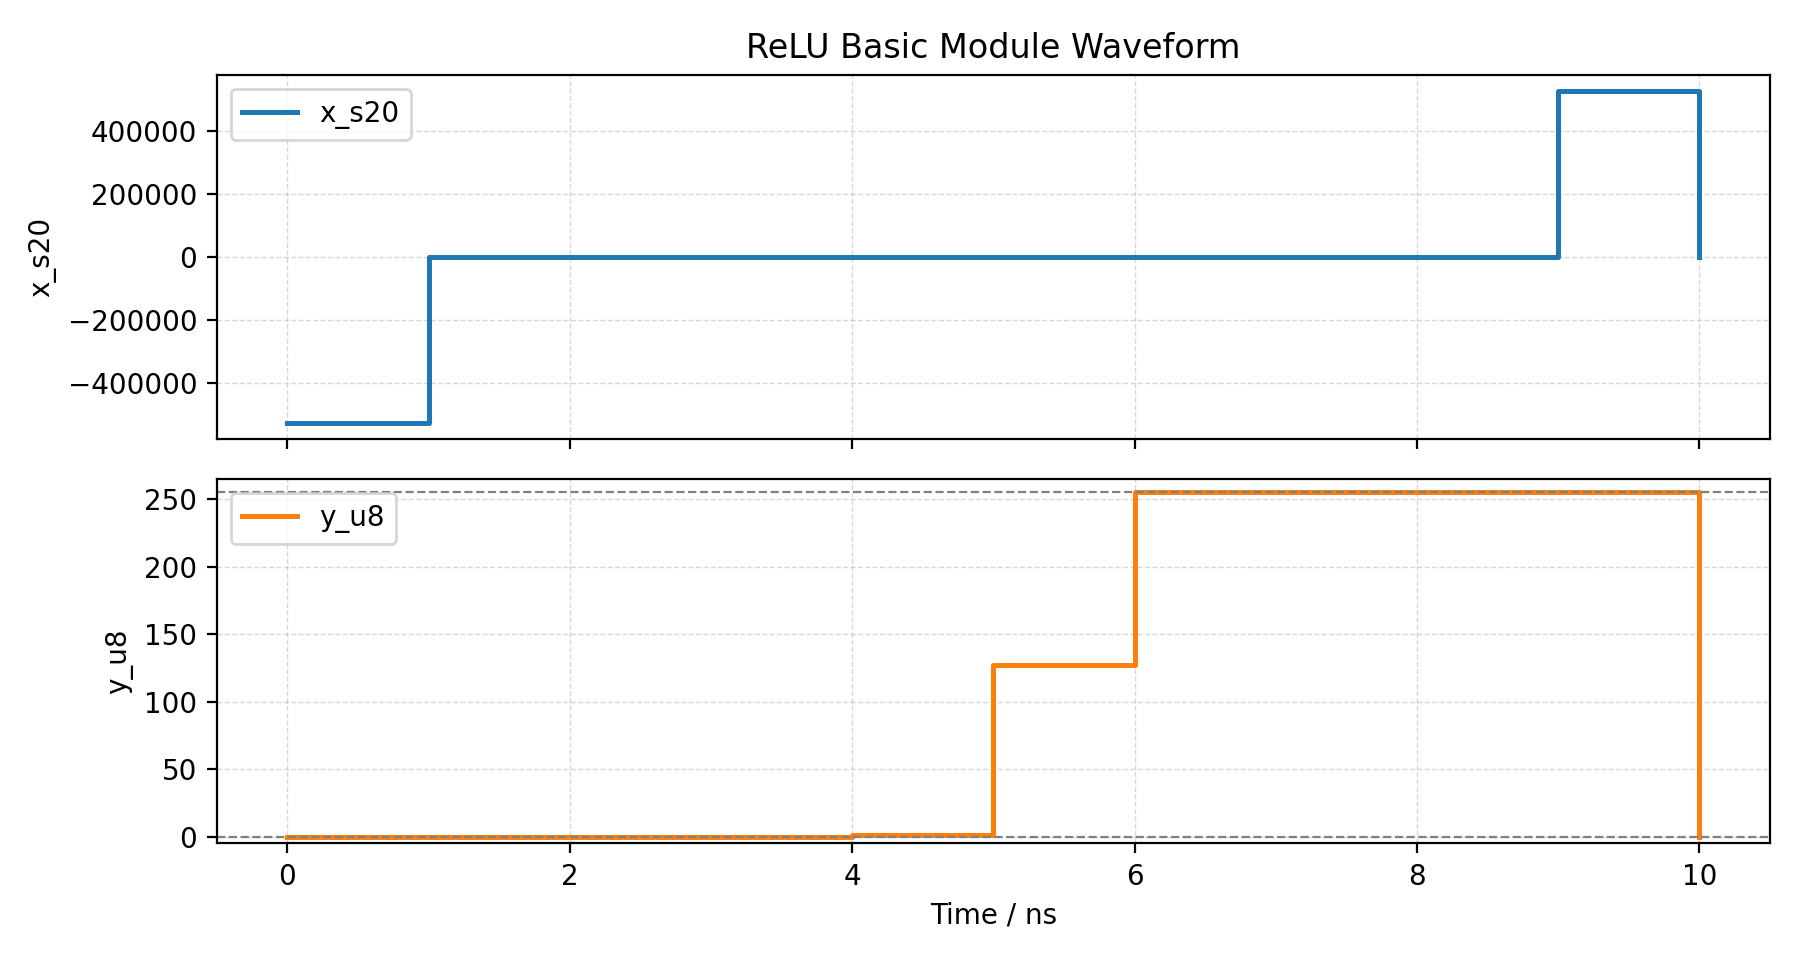
\includegraphics[width=0.92\textwidth]{figures/wave_relu_basic.png}
  \caption{基础模块波形：\texttt{relu\_s20} 的截断与饱和行为}
  \label{fig:wave-relu}
\end{figure}

\section{里程碑2：链式运算器集成与系统仿真}
\subsection{链式运算器的独立实现}
本次5个实验组全部以独立顶层模块存在，结构差异如下：
\begin{itemize}
  \item 第 1 组与第 2 组共享串行状态机框架，区别仅在于卷积阶段使用 \texttt{mul8} 还是 \texttt{mul8\_booth\_wallace}；
  \item 第 3 组采用独立的 BoothWallace + SIMD 数据通路，卷积结果、ReLU 与池化全部在同一条 32 位 SIMD 路径中完成；
  \item 第 4 组在第 3 组基础上加入固定 3 级数据流水，级间顺序为 ``卷积结果寄存 $\rightarrow$ ReLU 结果寄存 $\rightarrow$ 池化/输出寄存''；
  \item 第 5 组复用第 4 组流水结构，仅将第 1 级 SIMD 乘法阵列替换为显式 DSP48E1 实现。
\end{itemize}

\sourcecode{顶层 \texttt{cnn\_compare\_base\_top} 的 Verilog 源码}{../src/baseline/cnn_compare_base_top.v}
\sourcecode{顶层 \texttt{cnn\_compare\_booth\_top} 的 Verilog 源码}{../src/optimized/cnn_compare_booth_top.v}
\sourcecode{模块 \texttt{cnn\_chain\_core\_base} 的 Verilog 源码}{../src/baseline/cnn_chain_core_base.v}

\clearpage
\sourcecode{顶层 \texttt{cnn\_compare\_booth\_simd\_top} 的 Verilog 源码}{../src/optimized/cnn_compare_booth_simd_top.v}
\sourcecode{顶层 \texttt{cnn\_compare\_booth\_simd\_pipe\_top} 的 Verilog 源码}{../src/optimized/cnn_compare_booth_simd_pipe_top.v}
\sourcecode{顶层 \texttt{cnn\_compare\_booth\_simd\_pipe\_dsp\_top} 的 Verilog 源码}{../src/optimized/cnn_compare_booth_simd_pipe_dsp_top.v}
\sourcecode{模块 \texttt{cnn\_chain\_core\_booth\_simd} 的 Verilog 源码}{../src/optimized/cnn_chain_core_booth_simd.v}
\sourcecode{模块 \texttt{cnn\_chain\_core\_booth\_simd\_pipe} 的 Verilog 源码}{../src/optimized/cnn_chain_core_booth_simd_pipe.v}
\sourcecode{模块 \texttt{cnn\_chain\_core\_booth\_simd\_pipe\_dsp} 的 Verilog 源码}{../src/optimized/cnn_chain_core_booth_simd_pipe_dsp.v}
\sourcecode{共享卷积核心 \texttt{cnn\_conv3x3\_simd\_core} 的 Verilog 源码}{../src/optimized/cnn_conv3x3_simd_core.v}

\subsection{标准样例与手算结果}
系统 testbench \texttt{tb\_cnn\_core} 采用如下标准输入：
\begin{itemize}
  \item 图像矩阵为从 1 到 25 的顺序数列，按行优先排布为 $5\times 5$；
  \item 卷积核 9 个元素均为 1。
\end{itemize}

对应的卷积结果为：
\[
\begin{bmatrix}
63 & 72 & 81 \\
108 & 117 & 126 \\
153 & 162 & 171
\end{bmatrix}
\]
ReLU 后保持不变。继续执行 $2\times 2$ 平均池化，可得到：
\[
\begin{bmatrix}
90 & 99 \\
135 & 144
\end{bmatrix}
\]
在 \texttt{out\_flat\_u8x4} 中，该结果被打包为 \texttt{32'h9087635A}。

\subsection{系统仿真结果}
系统级仿真命令为：
\begin{verbatim}
powershell -ExecutionPolicy Bypass -File .\scripts\run_vivado_sim.ps1 -Mode system
\end{verbatim}

\texttt{tb\_cnn\_core} 对 5 个顶层分别拉起 \texttt{start}，并显式检查输出与延迟行为。结果如表 \ref{tab:sim-system} 所示。

\begin{table}[H]
\centering
\caption{系统级仿真结果}
\label{tab:sim-system}
\begin{tabular}{lccc}
\toprule
实验组 & 输出结果 & 延迟周期 \\
\midrule
串行 &  \texttt{32'h9087635A} & 96 \\
串行 + BoothWallace &  \texttt{32'h9087635A} & 96 \\
BoothWallace + SIMD &  \texttt{32'h9087635A} & 1 \\
BoothWallace + SIMD + 流水线 &  \texttt{32'h9087635A} & 3 \\
DSP 替换版 &  \texttt{32'h9087635A} & 3 \\
\bottomrule
\end{tabular}
\end{table}

XSIM 日志中可以直接看到如下 PASS 信息：
\begin{verbatim}
CASE=1 PASS cycles=96 out=9087635a
CASE=2 PASS cycles=96 out=9087635a
CASE=3 PASS cycles=1  out=9087635a
CASE=4 PASS cycles=3  out=9087635a
CASE=5 PASS cycles=3  out=9087635a
ALL TESTS PASSED.
\end{verbatim}

下面给出系统级 testbench 的完整 Verilog 源码。

\clearpage
\sourcecode{系统级 testbench \texttt{tb\_cnn\_core} 的 Verilog 源码}{../sim/tb_cnn_core.v}

\subsection{系统级与流水线波形}
图 \ref{fig:wave-system} 展示了 5 个独立顶层在同一 testbench 中的 \texttt{start}/\texttt{done} 时序对比，可以直观看到 96 周期、1 周期与 3 周期三类不同延迟行为。

\begin{figure}[H]
  \centering
  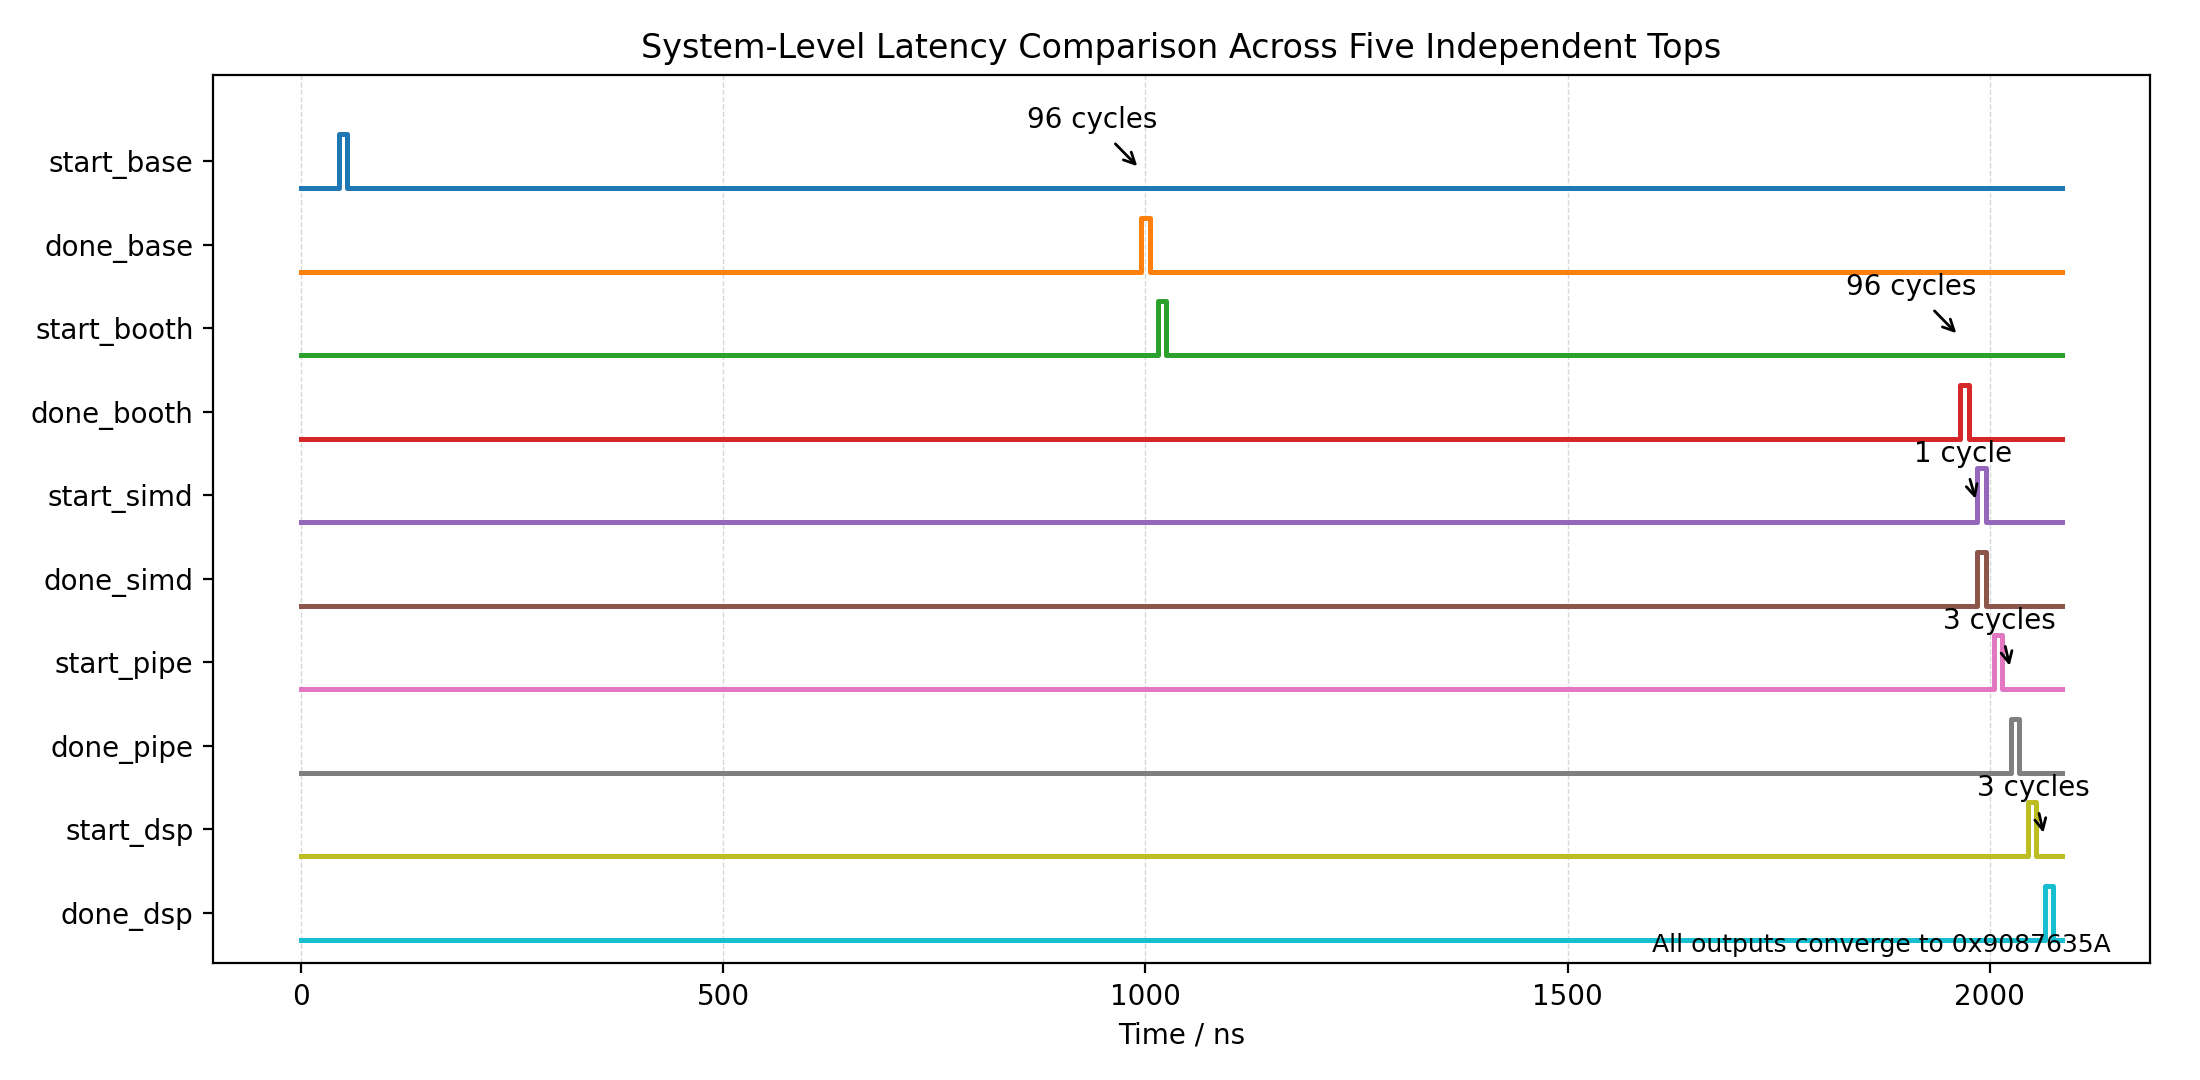
\includegraphics[width=\textwidth]{figures/wave_system_latency.png}
  \caption{系统级波形：5 个独立顶层的 \texttt{start}/\texttt{done} 延迟对比}
  \label{fig:wave-system}
\end{figure}

图 \ref{fig:wave-pipe} 给出了第 4 组流水线版本的关键内部波形。可以看到 \texttt{vld\_pipe} 按 \texttt{001 $\rightarrow$ 010 $\rightarrow$ 100} 依次推进，卷积结果寄存、ReLU 结果寄存和池化输出寄存依次有效，最终在第 3 个周期输出 \texttt{0x9087635A}。

\begin{figure}[H]
  \centering
  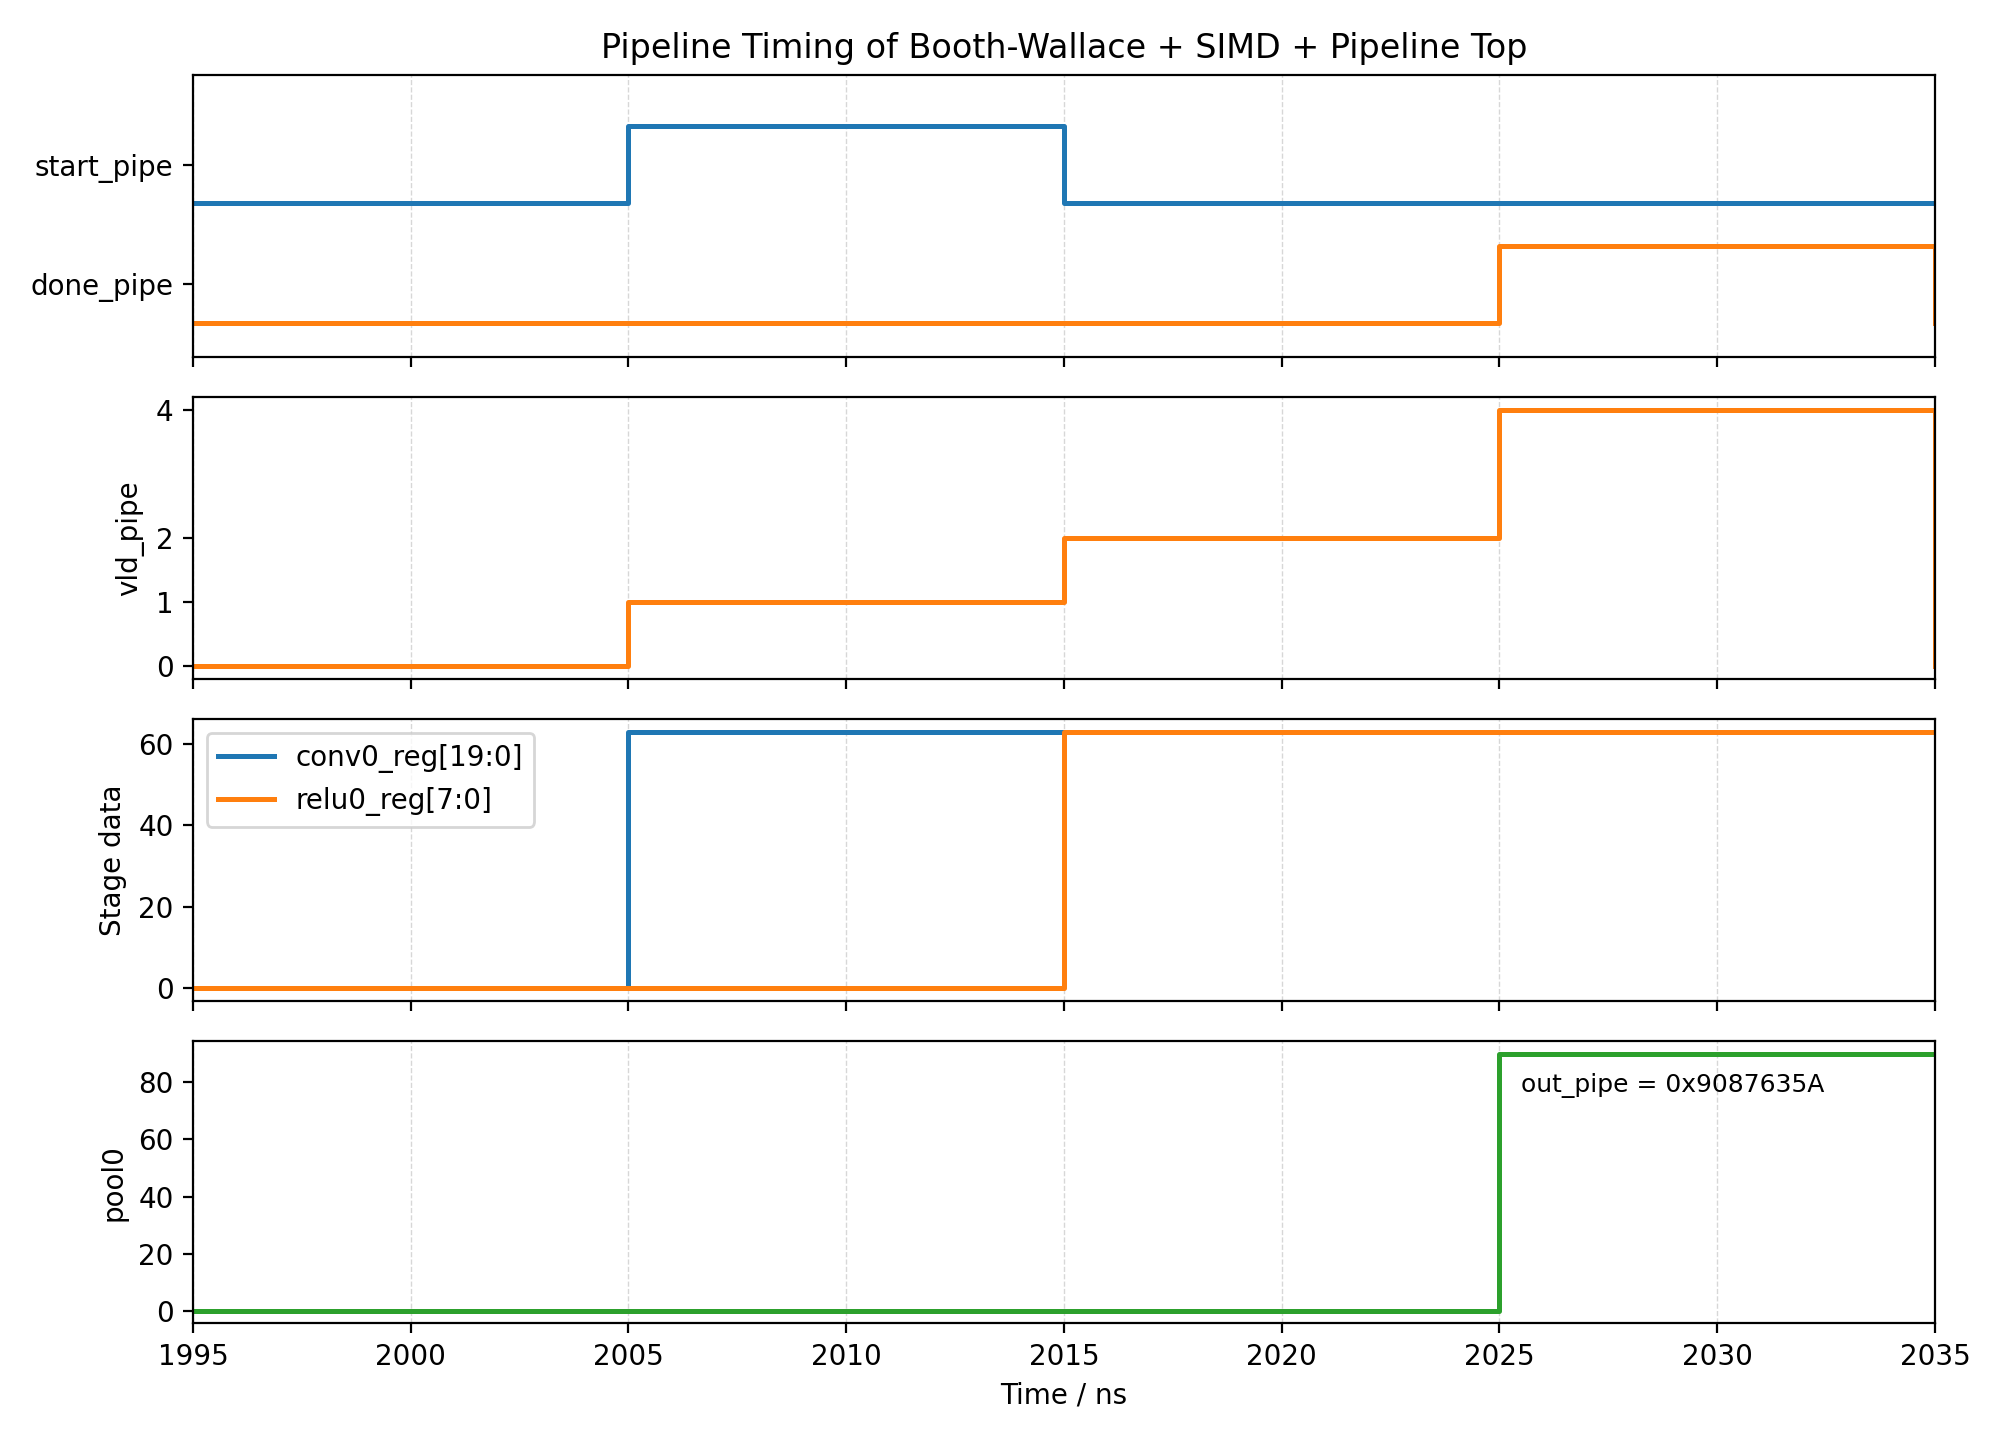
\includegraphics[width=\textwidth]{figures/wave_pipeline_timing.png}
  \caption{流水线波形：卷积寄存、ReLU 寄存与输出寄存的三级推进}
  \label{fig:wave-pipe}
\end{figure}

\section{里程碑3：优化与 Vivado 性能验证}
\subsection{综合设置}
综合脚本 \texttt{scripts/run\_vivado\_multi\_synth.tcl} 会依次对以下 5 个顶层执行 \texttt{synth\_design}：
\begin{itemize}
  \item \texttt{cnn\_compare\_base\_top}
  \item \texttt{cnn\_compare\_booth\_top}
  \item \texttt{cnn\_compare\_booth\_simd\_top}
  \item \texttt{cnn\_compare\_booth\_simd\_pipe\_top}
  \item \texttt{cnn\_compare\_booth\_simd\_pipe\_dsp\_top}
\end{itemize}

所有数据均来自 Vivado 2025.1 \texttt{utilization\_report} 与 \texttt{timing\_summary\_report}。

由于本报告在 5ns 约束下比较不同 RTL 结构，因此将估算最小时钟周期写为
\[
T_{\min} \approx 5.000 - \mathrm{WNS}
\]
再用
\[
f_{\max} \approx \frac{1000}{T_{\min}}
\]
估算最高工作频率，用于横向比较不同结构。

\subsection{主四组资源与时序对比}
主对比表仅统计前 4 组，不包含 DSP 替换版。结果如表 \ref{tab:main-compare} 所示。

\begin{table}[H]
\centering
\small
\caption{主四组实验的资源与时序对比}
\label{tab:main-compare}
\begin{tabular}{lrrrrrr}
\toprule
实验组 & LUT & FF & DSP & WNS/ns & 估算$f_{\max}$/MHz & 周期数 \\
\midrule
串行 & 550 & 304 & 0 & -5.546 & 94.82 & 96 \\
串行 + BoothWallace & 532 & 304 & 0 & -5.883 & 91.89 & 96 \\
BoothWallace + SIMD & 8095 & 33 & 0 & -6.030 & 90.66 & 1 \\
BoothWallace + SIMD + 流水线 & 8097 & 287 & 0 & -1.625 & 150.94 & 3 \\
\bottomrule
\end{tabular}
\end{table}

结合表 \ref{tab:main-compare} 与时序报告，可得到以下结论：
\begin{itemize}
  \item 第 2 组在串行框架中将 LUT 从 550 降到 532，但 WNS 从 -5.546\,ns 变为 -5.883\,ns，说明当前关键路径仍主要受串行卷积累加与布线影响，而不是单纯由乘法器级数决定；
  \item 第 3 组将计算周期压缩到 1 个周期，但由于卷积、激活和池化几乎全部落在同一条组合路径上，输入端口到输出寄存器的路径最长，WNS 反而最差；
  \item 第 4 组加入真实三级流水后，WNS 明显改善到 -1.625\,ns，估算最高频率提升到 150.94\,MHz，是主四组中时钟能力最强的实现；
  \item 若按估算频率折算单次计算时延，则第 1/2/3/4 组约为 1012.44\,ns、1044.73\,ns、11.03\,ns 和 19.88\,ns。也就是说，第 3 组在当前结构下具有更短的单次结果延迟，而第 4 组则以更好的时钟能力和更规则的吞吐结构取胜。
\end{itemize}

\begin{figure}[H]
  \centering
  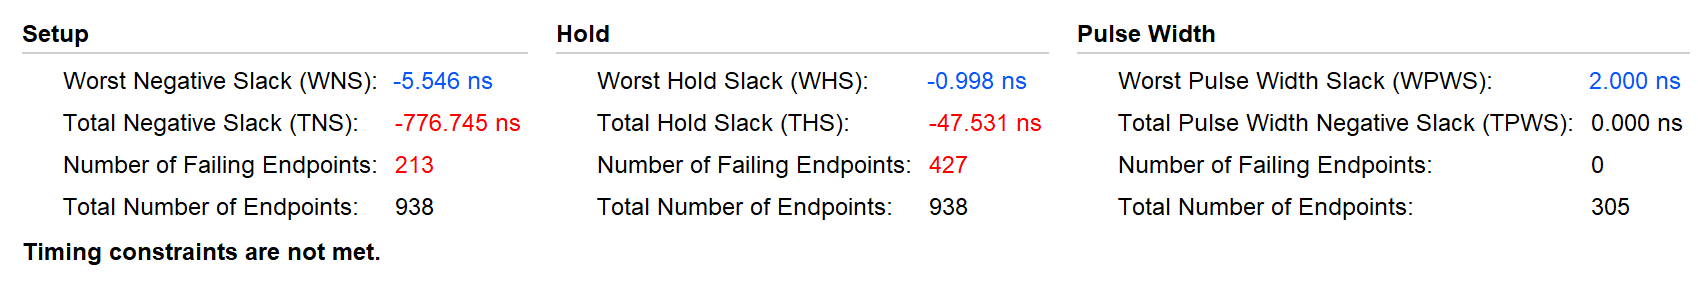
\includegraphics[width=\textwidth]{figures/time1.png}
  \caption{第一组实验的时序报告}
  \label{fig:time1}
\end{figure}
\begin{figure}[H]
  \centering
  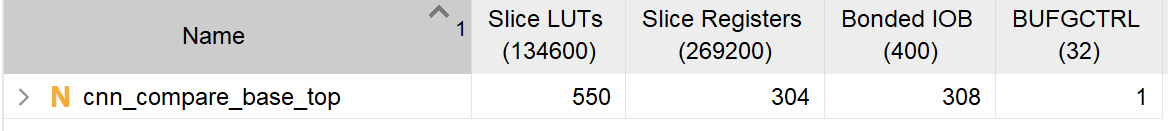
\includegraphics[width=\textwidth]{figures/util1.png}
  \caption{第一组实验的综合报告}
  \label{fig:util1}
\end{figure}

\begin{figure}[H]
  \centering
  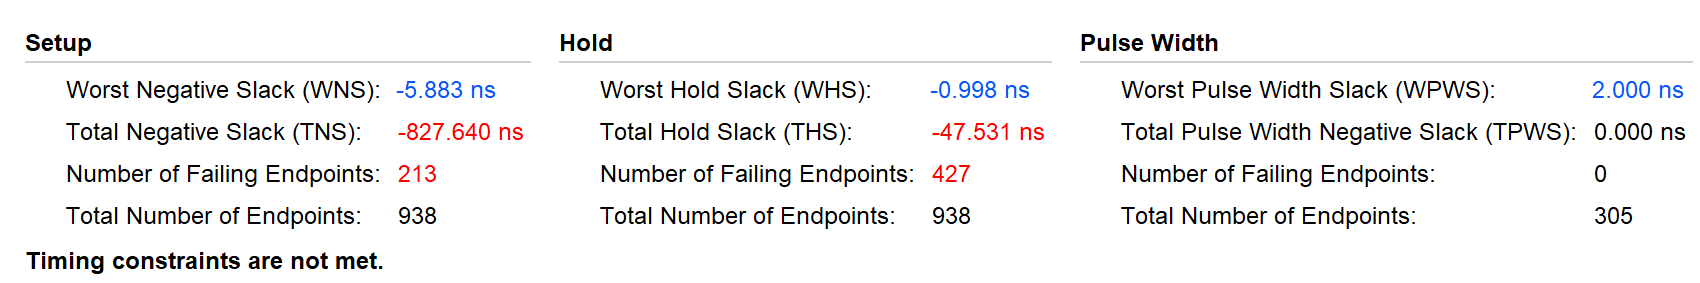
\includegraphics[width=\textwidth]{figures/time2.png}
  \caption{第二组实验的时序报告}
  \label{fig:time2}
\end{figure}

\begin{figure}[H]
  \centering
  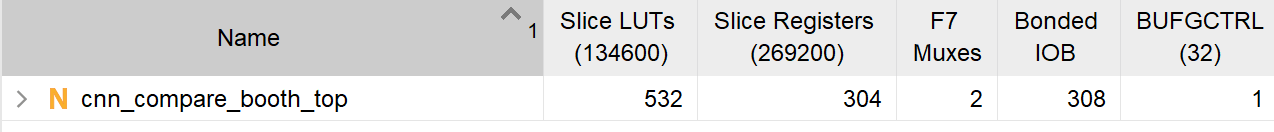
\includegraphics[width=\textwidth]{figures/util2.png}
  \caption{第二组实验的综合报告}
  \label{fig:util2}
\end{figure}

\begin{figure}[H]
  \centering
  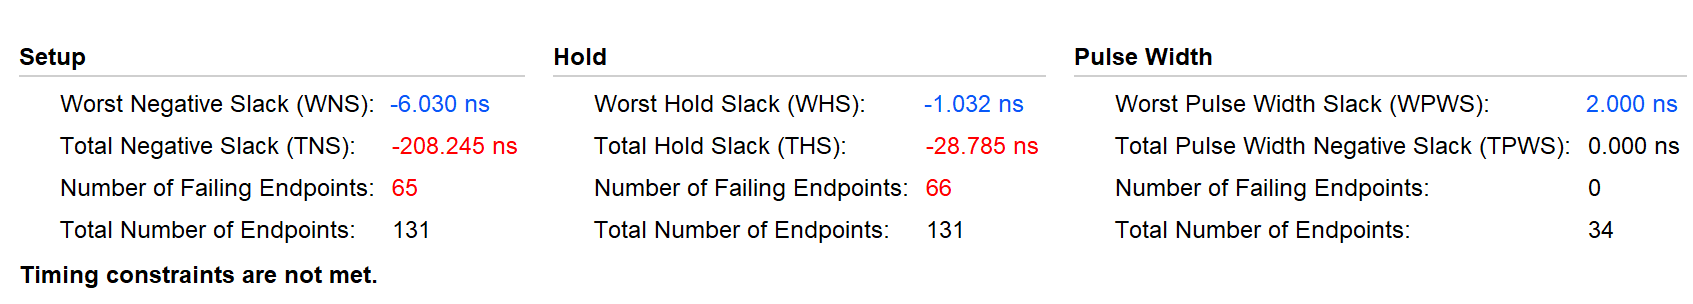
\includegraphics[width=\textwidth]{figures/time3.png}
  \caption{第三组实验的时序报告}
  \label{fig:time3}
\end{figure}

\begin{figure}[H]
  \centering
  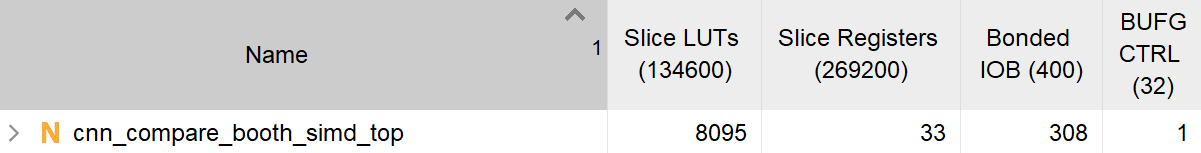
\includegraphics[width=\textwidth]{figures/util3.png}
  \caption{第三组实验的综合报告}
  \label{fig:util3}
\end{figure}


\begin{figure}[H]
  \centering
  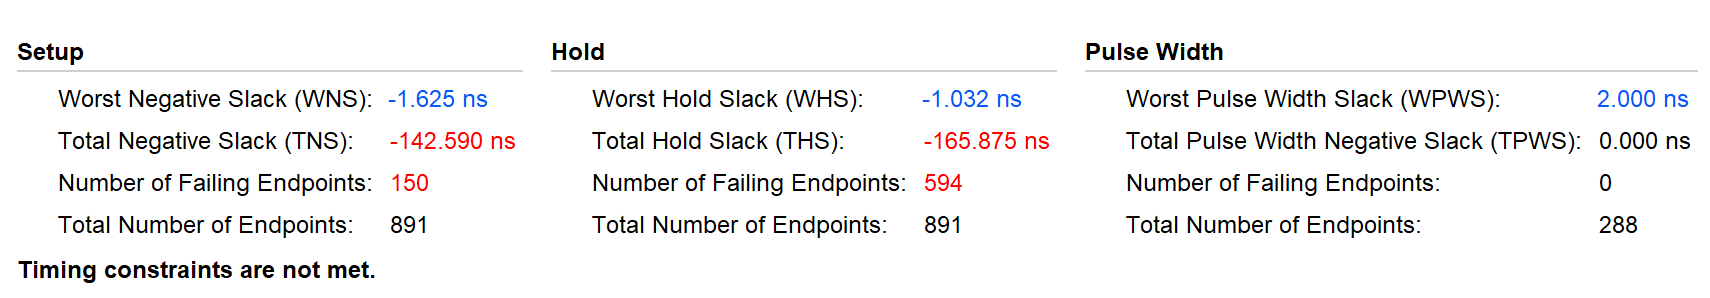
\includegraphics[width=\textwidth]{figures/time4.png}
  \caption{第四组实验的时序报告}
  \label{fig:time4}
\end{figure}

\begin{figure}[H]
  \centering
  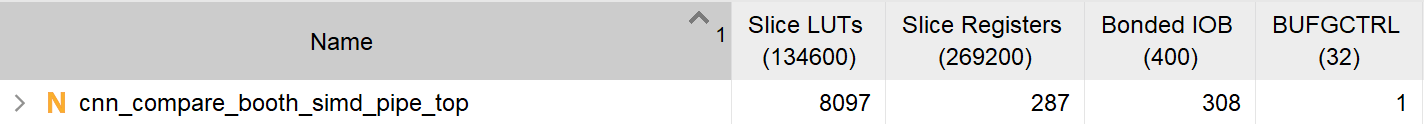
\includegraphics[width=\textwidth]{figures/util4.png}
  \caption{第四组实验的综合报告}
  \label{fig:util4}
\end{figure}

\subsection{第5组：在第4组基础上换用 DSP}
第 5 组仅作为第 4 组的 DSP 替换对照，不进入主四组主表。其比较结果如表 \ref{tab:dsp-compare} 所示。

\begin{table}[H]
\centering
\caption{第 4 组与第 5 组对比}
\label{tab:dsp-compare}
\begin{tabular}{lcc}
\toprule
指标 & 第 4 组：BoothWallace + SIMD + 流水线 & 第 5 组：DSP 替换版 \\
\midrule
LUT & 8097 & 1372 \\
FF & 287 & 287 \\
DSP & 0 & 81 \\
WNS/ns & -1.625 & -2.054 \\
估算$f_{\max}$/MHz & 150.94 & 141.76 \\
系统仿真周期数 & 3 & 3 \\
\bottomrule
\end{tabular}
\end{table}

这一组实验的结论比较明确：
\begin{itemize}
  \item 换用 DSP48E1 后，LUT 从 8097 大幅下降到 1372，逻辑资源减少约 83.1\%；
  \item 但在当前 200\,MHz 约束下，DSP 版的 WNS 并没有改善，反而从 -1.625\,ns 变为 -2.054\,ns；
  \item 功能与延迟周期保持不变，说明第 5 组达成了 ``只改实现、不改功能'' 的目标；
  \item 因此，对本工程当前 RTL 而言，DSP 替换带来的主要收益是逻辑资源迁移，而不是直接的性能提升。
\end{itemize}

\begin{figure}[H]
  \centering
  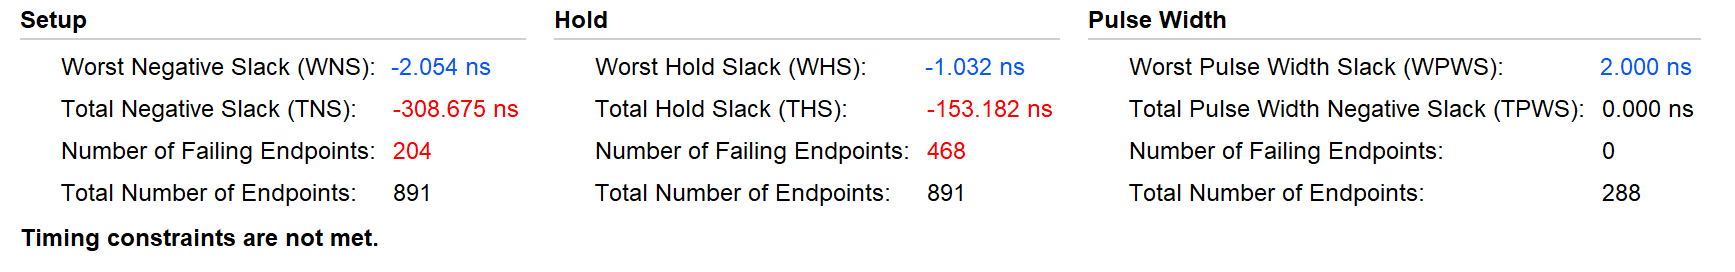
\includegraphics[width=\textwidth]{figures/time5.png}
  \caption{第五组实验的时序报告}
  \label{fig:time5}
\end{figure}

\begin{figure}[H]
  \centering
  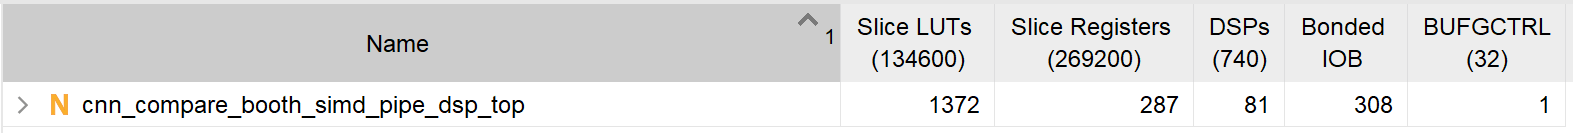
\includegraphics[width=\textwidth]{figures/util5.png}
  \caption{第五组实验的综合报告}
  \label{fig:util5}
\end{figure}


\section{实验收获}
\begin{itemize}
  \item 完整实现并验证了 8 位定点卷积、ReLU 激活和平均池化三段链路，对 CNN 基础算子在 FPGA 上的组织方式有了更具体的理解。
  \item 通过把 5 组实验拆成独立顶层，进一步体会到 ``便于综合分析的结构'' 与 ``便于功能复用的结构'' 并不总是同一件事。
  \item BoothWallace 乘法器、SIMD 路径和 3 级流水线都已经在工程中落地，并通过统一 testbench 验证了功能一致性。
  \item 从 Vivado 报告中可以看出，优化并不总会直接转化为更高主频；关键路径位置、寄存器边界和布线代价同样会改变最终结果。
  \item DSP 替换版说明了另一类典型工程取舍：它显著降低了 LUT 占用，但在当前结构下并未直接带来性能收益。
\end{itemize}

\section{附：源码目录}
\begin{itemize}
  \item \verb|project1/src/baseline/|：串行基线实现，包括 \verb|mul8.v|、\verb|add8.v|、\verb|relu_s20.v|、\verb|div4.v|、\verb|cnn_chain_core_base.v| 等；
  \item \verb|project1/src/optimized/|：BoothWallace、SIMD、流水线和 DSP 版本实现；
  \item \verb|project1/sim/|：模块级与系统级 testbench；
  \item \verb|project1/scripts/run_vivado_sim.ps1|：Vivado/XSIM 仿真入口；
  \item \verb|project1/scripts/run_vivado_multi_synth.tcl|：5 个顶层的综合入口；
  \item \verb|project1/scripts/export_wave_figures.py|：从 VCD 导出报告波形图；
  \item \verb|project1/constraints/project1.xdc|：时钟与 I/O 约束；
  \item \verb|project1/report/figures/|：报告中引用的代表性波形图片。
\end{itemize}

\end{document}
